% !TEX root = ../main.tex
\section{Integrity vs.\ Income-modellen}\label{thr:integrity-vs-income-model}

\paragraph{Definisjon.} BSZ kap.\ 2 presenterer en nyttemodell der medarbeideren velger mellom to ``goder'': \emph{integritet} (etisk atferd, regeloverholdelse) og \emph{indkomst} (personlig inntekt/bonus). Kompensasjonsplanens design endrer budsjettbetingelsen og dermed agentens optimale valg -- selv for en agent som verdsetter integritet, kan et dårlig designet insentivsystem vippe valget mot uetisk atferd. [SLIDE]

\subsection*{Forklaring}

Modellen bruker standard mikroøkonomisk rammeverk (indifferenskurver + budsjettlinje) overført til et ikke-standard godsrom: integritet og indkomst. [SLIDE/BOK]

\textbf{Akser:}
\begin{itemize}\setlength{\itemsep}{1pt}
\item \textbf{Horisontal:} Integritet (fra lav til høy; mer integritet = mer regeloverholdelse, mindre juks).
\item \textbf{Vertikal:} Indkomst (personlig inntekt/bonus).
\end{itemize}

\textbf{Indifferenskurver:} Agenten har preferanser over begge goder. Indifferenskurvene er konvekse mot origo: agenten er villig til å bytte noe integritet mot mer inntekt (og omvendt). MRS mellom indkomst og integritet varierer -- noen verdsetter integritet høyt (bratte kurver), andre lavt (flate kurver). [BOK]

\textbf{Budsjettlinje (opportunity set):} Kompensasjonsplanen definerer hvilke kombinasjoner av integritet og indkomst som er tilgjengelige:
\begin{itemize}\setlength{\itemsep}{2pt}
\item \textbf{Før aggressivt insentivsystem:} Budsjettlinjen er relativt flat -- inntektsforskjellen mellom ``jukse'' og ``ikke jukse'' er liten. Agenten velger høy integritet.
\item \textbf{Etter aggressivt insentivsystem:} Budsjettlinjen roterer utover -- inntektsgevinsten ved å jukse (fire kunder, ta snarveier, falske salg) øker dramatisk. Agenten kan nå oppnå mye høyere inntekt ved å ofre integritet.
\item \textbf{Resultat:} Tangentpunktet mellom indifferenskurve og budsjettlinje skifter mot lavere integritet og høyere inntekt.
\end{itemize}

\textbf{Nøkkelinnsikt:} Kompensasjonsdesign er ikke bare et spørsmål om å ``motivere innsats'' -- det påvirker \emph{hva slags} innsats som velges. En kontrakt med høy $\beta$ på enkelt målbare resultater (salg, antall kontoer) uten sjekk på kvalitet/etikk dreier agenten bort fra integritet. [SLIDE]

\subsection*{Grafisk modell}

\begin{figure}[H]
  \centering
  
\includegraphics[width=0.35\linewidth]{BSZ_kap_2_2026/by_slide/slide_005/BSZ_kap_2_2026_slide_005_asset_01_image4.png}
  \caption{Metafor: pengeankret drar agenten ned. Et aggressivt insentivsystem øker den personlige kostnaden ved å forbli etisk -- selv en agent som verdsetter integritet, kan dras mot uetisk atferd når relativprisen mellom integritet og inntekt endres tilstrekkelig. (BSZ kap.\ 2, slide 5) [SLIDE]}
\end{figure}

\begin{figure}[H]
\centering
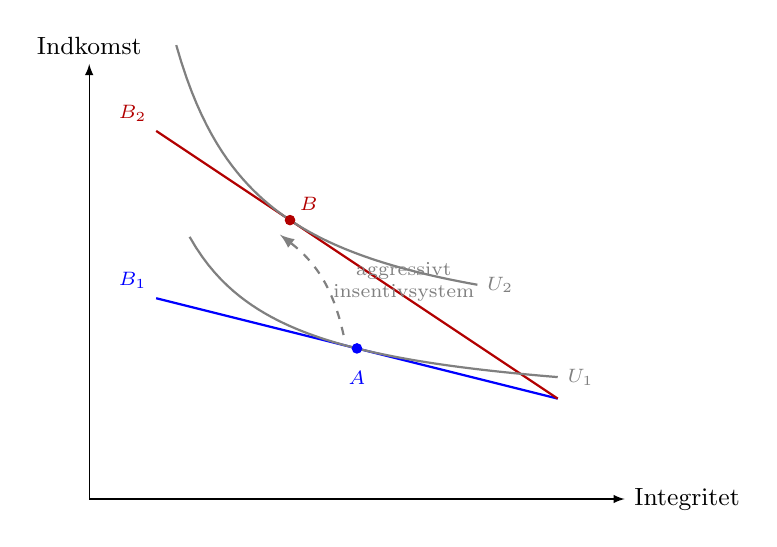
\begin{tikzpicture}[>=latex, scale=0.85, every node/.style={font=\small}]
  % Akser
  \draw[->] (0,0) -- (8,0) node[right] {Integritet};
  \draw[->] (0,0) -- (0,6.5) node[above] {Indkomst};
  % Budsjettlinje 1 (moderat insentiv)
  \draw[thick, blue] (1.0,3.0) -- (7.0,1.5);
  \node[blue, above left, font=\scriptsize] at (1.0,3.0) {$B_1$};
  % Budsjettlinje 2 (aggressivt insentiv - rotert)
  \draw[thick, red!70!black] (1.0,5.5) -- (7.0,1.5);
  \node[red!70!black, above left, font=\scriptsize] at (1.0,5.5) {$B_2$};
  % Indifferenskurve U1: y = 4/x + 1.25, tangent til B1 i (4, 2.25)
  \draw[thick, gray, domain=1.5:7.0, samples=60]
    plot (\x, {4/\x + 1.25});
  \node[gray, right, font=\scriptsize] at (7.0,1.82) {$U_1$};
  % Indifferenskurve U2: y = 6/x + 13/6, tangent til B2 i (3, 25/6)
  \draw[thick, gray, domain=1.3:5.8, samples=60]
    plot (\x, {6/\x + 13/6});
  \node[gray, right, font=\scriptsize] at (5.8,3.20) {$U_2$};
  % Tangent A (høy integritet, B1) ved (4, 2.25)
  \filldraw[blue] (4.0,2.25) circle (2pt);
  \node[below, blue, font=\bfseries\scriptsize] at (4.0,2.05) {$A$};
  % Tangent B (lav integritet, B2) ved (3, 25/6 ~ 4.167)
  \filldraw[red!70!black] (3.0,4.167) circle (2pt);
  \node[above right, red!70!black, font=\bfseries\scriptsize] at (3.0,4.167) {$B$};
  % Annotations
  \draw[->, thick, dashed, gray] (3.8,2.45) to[bend right=20] (2.85,3.95);
  \node[font=\scriptsize, gray, text width=2.5cm, align=center] at (4.7,3.25) {aggressivt\\insentiv\-system};
\end{tikzpicture}
\caption{\textbf{Integrity vs.\ Income.} Med moderat insentiv (blå $B_1$) velger agenten punkt $A$: høy integritet, moderat inntekt. Etter innføring av aggressivt prestasjonsbasert insentiv (rød $B_2$) roterer budsjettlinjen utover -- gevinsten ved å ofre integritet øker. Nytt optimum er punkt $B$: lav integritet, høy inntekt. Kompensasjonsdesignet endrer etisk atferd uten å endre preferanser. [SLIDE -- BSZ kap.\ 2]}
\end{figure}

\subsection*{Kjerneforutsetninger}
\begin{itemize}
\item Agenten har stabile preferanser som inkluderer integritet som et gode (ikke bare inntekt).
\item Kompensasjonsplanen endrer relativprisen mellom integritet og inntekt.
\item Integritet er \emph{ikke} perfekt overvåkbart -- ellers kunne prinsipalen kontraktfeste etikk direkte.
\item Standard nytteteori: konvekse indifferenskurver, monotone preferanser.
\end{itemize}

\subsection*{Muligheter}
\begin{itemize}
\item Forklarer corporate scandals som resultat av insentivsystem, ikke bare ``dårlige mennesker''.
\item Gir normativt verktøy: design kompensasjonsplaner som \emph{ikke} gjør det irrasjonelt å være etisk.
\item Viser at etikk og insentiver er komplementære designvariabler -- begge hører til den organisatoriske arkitekturen.
\item Kobler insentivdesign (\SThree) til kultur og governance.
\end{itemize}

\subsection*{Begrensninger og kritikk}
\begin{itemize}
\item ``Integritet'' som målbart gode er en sterk abstraksjon -- etiske valg er ofte binære (jukse/ikke jukse), ikke kontinuerlige.
\item Modellen ignorerer sosiale normer, gruppepress og culture som påvirker atferd uavhengig av insentiver.
\item Forutsetter rasjonelt valg -- atferdsøkonomi viser at etiske valg ofte er intuitive, ikke kalkulerte.
\item Alternativ forklaring: insentiver kan \emph{crowde ut} indre motivasjon (Frey \& Jegen 2001) -- noe modellen ikke fanger.
\end{itemize}

\subsection*{Eksempler}
\begin{itemize}\setlength{\itemsep}{2pt}
\item \textbf{Wells Fargo (2016):} Aggressive cross-sell-kvoter roterte budsjettlinjen kraftig -- bankansatte valgte punkt $B$: 3{,}5 mill.\ falske kontoer. Etter skandalen reduserte Wells Fargo $\beta$ og innførte kvalitative mål -- budsjettlinjen roterte tilbake. [EKS]
\item \textbf{Enron (2001):} Mark-to-market-basert bonus ga enormt insentiv til å oppblåse verdier. Ansatte med ellers god integritet justerte estimater aggressivt fordi budsjettlinjen premiertete det. [EKS]
\item \textbf{Skandinaviske banker etter hvitvaskingsskandalene (Danske Bank, Swedbank):} Compliance-kultur styrket og bonusandelen redusert -- budsjettlinjen rotert tilbake mot integritet. [EKS]
\end{itemize}

\subsection*{Kobling til søyle og andre teorier}
Søyle: \SThree\ (kompensasjonsdesign påvirker etisk atferd), \STwo\ (hva som måles bestemmer hva som belønnes). Relaterte: \thref{incentive-coefficient}{Incentive coefficient} ($\beta$ driver rotasjonen), \thref{moral-hazard}{Moral hazard}, \thref{principal-agent}{Principal-agent}, \thref{gaming-in-performance-measurement}{Gaming} (integrity--income-trade-offen er en form for gaming), \thref{risk-expected-value-model}{Risk--expected value-modellen} (den andre nyttemodellen i Q15).

\paragraph{Brukt i spørsmål:} Q15.
